\subsection{Rate monotonic scheduling}
Rate monotonic scheduling (RMS) is a preemptive scheduling algorithm used when you have set of strictly periodic tasks with deadlines equal to their periods. A number of other assumptions are also required. All of them are listed here.
\begin{itemize}
\item Single processor
\item Task deadlines are equal to their periods
\item Periodic tasks
\item All tasks are released as soon as they arrive
\item All tasks start at the same time
\item All tasks are independent
\item No precedence or resource constraints
\item No task can suspend itself
\item All overheads in the kernel are assumed to be zero
\end{itemize}

\subsection{Schedulability}
To determine schedulability of a task set, a utilization test is applied. The formal version of the test is as follows:

\begin{equation}
\displaystyle\sum\limits_{i=1}^{n} \frac{C_i}{T_i} \leq n \left( 2^{\frac{1}{n}} - 1 \right) 
\end{equation}
Or, in other words: The cpu usage represented on the left hand side by the sum of all the individual tasks utilization of the cpu in their period must be less that $n \left( 2^{\frac{1}{n}} - 1 \right) $, where $n$ is the number of tasks.\\
This is a sufficient test, and task sets that fail this test are not necessarily unschedulable.\\\\
Futhermore, it holds that:
\begin{equation}
\underset{y\rightarrow0}{\lim}U_{lub}(n)=\ln2
\end{equation}
Proven by Liu and Leyland.

\subsection{Simulation}
%REMEBER! THIS IS A SIMULATOR - Simulate the running of an embedded application on a single processor system using preemtive fixed-priority scheduling.
For simulating a task set under rate monotonic scheduling, we first have to find a LCM of all the periods for the tasks in the set. This is also known as the hyperperiod. As $C_i$ needs to be randomized, the simulation should run for a number multiples of the hyperperiod. The multiple of LCM will be denoted $n$
\subsubsection*{Priority assignment}
The priorities is in RMS defined as the inverse of the period. In this implementation, the priority is relative to the hyperperiod and defined as $P_i = \frac{LCM}{T_i}$. This is done to avoid rounding errors and floating point arithmetic in simulation.
\subsubsection*{Job initialization}
To initialize the jobs we insert them into a job queue with release time equal to $\tau_{i}.period \cdot (j - 1)$ where $\tau_i$ is the task of the job, and $j$ is j'th occurrence of the task. The job's time  (remaining execution time) is also randomized in this step.
\subsubsection*{Simulation}
The jobs are sorted on start time and priority, and the simulation runs by going through each cycle from 1 to $n$. In each cycle, a list of ready jobs are generated and the job with the highest priority is picked to execute. Ready jobs are jobs that have time > 0 and release < current cycle.\\
Execution is done by a tick method call to the job that decreases time.\\
When the job terminates (time = 0), the response time is recorded and compared to the overall worst-case response time of the task, recording if it is worse that any previous.

\subsection{Output}
The simulator produces a textual output in the form:(name) (WCRT) newline. An example is shown below:
\begin{verbatim}
T1 1
T2 54
T3 2
T4 4
T5 6
T6 10
T7 28
\end{verbatim}
It also returns the schedulability determined by asserting $D_i > WCRT_i$ for each task:
\begin{verbatim}
Simulator.RateMonotonicSimulation Reports Schedulable
\end{verbatim}
In addition the simulator also produces a graphical output in the form of a timeline in svg format. An example is shown i figure \ref{fig:example_timeline_output}

\begin{figure}[h]
\centering
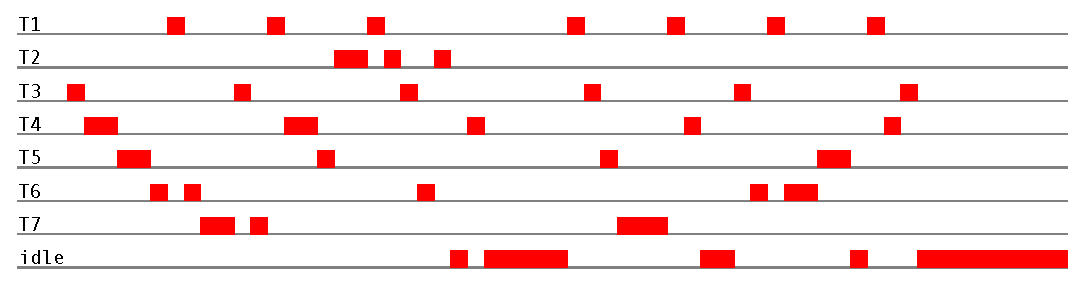
\epsfig{file=fig/example_timeline.eps, height=0.8in}
\caption{Example timeline}
\label{fig:example_timeline_output}
\end{figure}

\subsection{Implementation details}
\subsubsection{Generation of the random numbers}
In order to perform a simulation having both a BCET and WCET, a randomization is needed. For this simulators purpose, either uniform or Gaussian distribution is used, depending on the configuration parameters. On an implementation note, Java's is used java.util.Random class is used for generating the random numbers. When using the uniform distribution the following should be taken into account:

\begin{quotation}
... Returns a pseudorandom, uniformly distributed int value between 0 (inclusive) and the specified value (exclusive) ... All n possible int values are produced with (approximately) equal probability\cite{javadoc16}
\end{quotation}
%TODO set qoute origin

As the upper value is exclusive, we need a value in the range $[BCET:WCET+1[$ when using a uniform distribution.\\
Future improvement could also include to possibility to use a seed, to be able to recreate the random numbers generated.

\subsubsection{Traceability}
To be able to determine the situation of the first time overflow, a timeline is maintained, raising a global flag when the overflow occurs, and record the cycle.\\
%Can you determine what situation created the worst-case response time for a particular task (what other tasks interrupted it, when, and for how long)?
To be able to trace what other task interrupted it, we can go back to the point where the overflown task last stopped (in time) and record the tasks between them.

\subsubsection{Response time guarantee}
%Can you guarantee that the response time will not be larger than the worst-case numbers you get from the simulator?
When using random execution times are used for simulation, no guarantee can be provided. Although if you have a random distribution that is similar to the one in the actual application, then you are able give a better estimate.\\

% What happens if you simulate using the execution time equal to WCET?
When the execution time is always set to WCET, You end up with a very pessimistic estimate on the response time - although guaranteed to be accurate. In praxis, a lot of CPU time will be wasted, especially if the execution time is much larger than the typical execution and only happens in very rare or perhaps even in theoretical cases.\\
Effectively you get the same figures as the response time analysis explained in section \ref{sec:rta}.
\subsection{Final thoughts}
Although one of the assumptions is that tasks must be independent, it is not guaranteed that task are statistically independent - meaning that a higher execution time on one task can be due to an external effect, that affects other tasks as well.\\
This eventually leads to a cascade of higher response times on all tasks that depend on, for example, some external input. Due to, that in the real world variables are not always independent.